\documentclass[a4paper]{article}

%use the english line for english reports
%usepackage[english]{babel}
\usepackage[portuguese]{babel}
\usepackage[utf8]{inputenc}
\usepackage{indentfirst}
\usepackage{graphicx}
\usepackage{verbatim}


\begin{document}

\setlength{\textwidth}{16cm}
\setlength{\textheight}{22cm}

\title{\Huge\textbf{FABRIK}\linebreak\linebreak\linebreak
\Large\textbf{Relatório Intercalar}\linebreak\linebreak
\linebreak\linebreak

\includegraphics[scale=0.1]{feup-logo.png}\linebreak\linebreak
\linebreak\linebreak
\Large{Mestrado Integrado em Engenharia Informática e Computação} \linebreak\linebreak
\Large{Programação em Lógica}\linebreak
}

\author{\textbf{Grupo Fabrik_3:}\\
André Cruz - up201503776@fe.up.pt \\
Edgar Carneiro - up201503784@fe.up.pt \\
\linebreak\linebreak \\
 \\ Faculdade de Engenharia da Universidade do Porto \\ Rua Roberto Frias, s\/n, 4200-465 Porto, Portugal \linebreak\linebreak\linebreak
\linebreak\linebreak\vspace{1cm}}

\maketitle
\thispagestyle{empty}

%************************************************************************************************
%************************************************************************************************

\newpage

%Todas as figuras devem ser referidas no texto. %\ref{fig:codigoFigura}
%
%%Exemplo de código para inserção de figuras
%%\begin{figure}[h!]
%%\begin{center}
%%escolher entre uma das seguintes três linhas:
%%\includegraphics[height=20cm,width=15cm]{path relativo da imagem}
%%\includegraphics[scale=0.5]{path relativo da imagem}
%%\includegraphics{path relativo da imagem}
%%\caption{legenda da figura}
%%\label{fig:codigoFigura}
%%\end{center}
%%\end{figure}
%
%
%\textit{Para escrever em itálico}
%\textbf{Para escrever em negrito}
%Para escrever em letra normal
%``Para escrever texto entre aspas''
%
%Para fazer parágrafo, deixar uma linha em branco.
%
%Como fazer bullet points:
%\begin{itemize}
	%\item Item1
	%\item Item2
%\end{itemize}
%
%Como enumerar itens:
%\begin{enumerate}
	%\item Item 1
	%\item Item 2
%\end{enumerate}
%
%\begin{quote}``Isto é uma citação''\end{quote}

%Index
\tableofcontents{}
\newpage

%%%%%%%%%%%%%%%%%%%%%%%%%%
\section{O Jogo}\textit{  Fabrik}

\subsection{História}
O jogo - \texti{Fabrik} - foi recentemente desenvolvido por Dieter Stein, em Agosto de 2017, como parte de um estudo para o desenvolvimento de um novo jogo, Urbino.

\subsection{Material}
\begin{itemize}
	\item Tabuleiro quadrangular
	\item Quantidade suficiente de peças pretas e brancas
	\item Duas peças vermelhas chamadas trabalhadores
\end{itemize}

\begin{figure}[h!]
\begin{center}
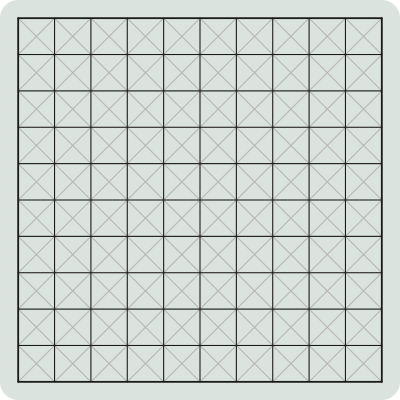
\includegraphics[height=20cm,width=15cm]{fabrik_empty_board.png}
%%\includegraphics[scale=0.5]{path relativo da imagem}
\caption{Tabuleiro vazio de 11 x 11 espaços}
\label{Figura 1}
\end{center}
\end{figure}

\subsection{Regras}
As pretas (jogador que joga com peças de cor preta) começam por colocar um dos trabalhadores num espaço á sua escolha. De seguida, as brancas (jogador que joga com peças de cor branca) coloca o outro trabalhador num espaço qualquer. As pretas decidem quem começa por jogar.
O jogo funciona por turnos sendo que em cada um turno um jogador pode, se assim optar, mexer um dos trabalhadores para um espaço vazio. De seguida, o jogador deve jogar uma das suas  peças e coloca-la num ponto de interseção entre as “linhas de visão dos dois trabalhadores”. As linhas de visão dos trabalhadores são as linhas na diagonal, horizontal e vertical sobre as quais os trabalhadores se encontram posicionados.

\begin{figure}[h!]
\begin{center}
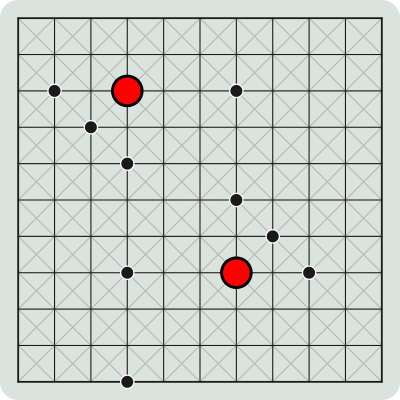
\includegraphics[height=20cm,width=15cm]{fabrik_intersection.png}
%%\includegraphics[scale=0.5]{path relativo da imagem}
\caption{Pontos de interseção entre os dois trabalhadores}
\label{Figura 2}
\end{center}
\end{figure}

No caso especial em que os dois trabalhadores se encontram sobre uma mesma linha ortogonal ou diagonal, apenas os espaços entre eles são considerados pontos de interseção (se estiverem vazios), ao invés da totalidade dessa linha.
Ganha o jogo o jogador que consiga criar uma linha de pelo menos 5 pedras da sua cor, ortogonalmente ou diagonalmente. Um jogador ganha também o jogo se o seu adversário não conseguir posicionar nenhum dos trabalhadores de forma a poder colocar uma pedra sua no tabuleiro.

\begin{figure}[h!]
\begin{center}
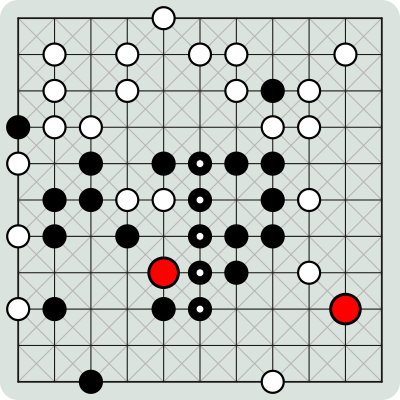
\includegraphics[height=20cm,width=15cm]{fabrik_full_board.png}
%%\includegraphics[scale=0.5]{path relativo da imagem}
\caption{Final de uma partida de Fabrik, com vitórias das pretas}
\label{Figura 3}
\end{center}
\end{figure}

\newpage


\section{Modelação do Jogo em Prolog}
%%%%%%%%%%%%%%%%%%%%%%%%%%
\subsection{Representação do Estado do Jogo}

Descrever a forma de representação do estado do tabuleiro (tipicamente uma lista de listas), com exemplificação em Prolog de posições iniciais do jogo, posições intermédias e finais, acompanhadas de imagens ilustrativas.

\newpage

%%%%%%%%%%%%%%%%%%%%%%%%%%
\subsection{Visualização do Tabuleiro}

Descrever a forma de visualização do tabuleiro em modo de texto e o(s) predicado(s) Prolog construídos para o efeito.
Deve ser incluída pelo menos uma imagem correspondente ao output produzido pelo predicado de visualização.

\newpage

%%%%%%%%%%%%%%%%%%%%%%%%%%
\subsection{Movimentos}

Elencar os movimentos (tipos de jogadas) possíveis e definir os cabeçalhos dos predicados que serão utilizados (ainda não precisam de estar implementados).


\end{document}
